\documentclass[12pt, a4paper]{article}

% Required packages
\usepackage{graphicx}
\usepackage{amsmath}
\usepackage{hyperref}
\usepackage{geometry}
\geometry{a4paper, margin=1in}

\title{\textbf{The Balam Protocol: Hardware-Agnostic Runtime Defense for Spiking Neural Networks}}
\author{\textbf{Asnain I Shaikh} \\ \textit{Deep-Tech Founder \& Security Researcher}}
\date{November 2026}

\begin{document}

\maketitle

\begin{abstract}
As edge computing shifts toward biological architectures, Brain-Computer Interfaces (BCIs) and autonomous robotics increasingly rely on Spiking Neural Networks (SNNs). However, these event-driven chips remain catastrophically vulnerable to physical Side-Channel Attacks, specifically Electromagnetic Fault Injection (EMFI). This paper introduces the Balam Protocol: a runtime firmware layer that mathematically filters malicious analog voltage glitches in real-time, preserving temporal membrane integrity without compromising ultra-low latency operations.
\end{abstract}

\section{The Threat Model: Digital Seizures}
Unlike traditional von Neumann architectures, SNNs do not rely on a global clock. They process asynchronous spikes. A hacker utilizing an EMFI tool can inject localized magnetic interference to artificially raise the membrane potential of a Leaky Integrate-and-Fire (LIF) neuron. This bypasses traditional software firewalls entirely, resulting in a continuous, uncontrollable spike train—a digital seizure that can cause kinetic destruction in edge devices.

\section{The Balam Architecture}
The Balam Protocol acts as a biological shield embedded before the synaptic computation layer. By continuously monitoring the incoming voltage against standard biological thresholds, it clamps malicious energy injections before they breach the membrane potential limits.

\subsection*{Mathematical Formulation}
The simulation utilizes a discrete-time Leaky Integrate-and-Fire (LIF) model, where the membrane potential $U[t]$ updates according to the following decay and input integration:
\begin{equation}
    U[t+1] = \beta U[t] + I[t] - S[t]\theta
\end{equation}
where $\beta$ is the decay rate, $I[t]$ is the incoming synaptic current, $S[t] \in \{0,1\}$ is the spike emission, and $\theta$ is the firing threshold.

During an EMFI attack, the anomalous current $I_{EMFI}[t] \gg \theta$, mathematically overwhelming the subtractive reset mechanism ($S[t]\theta$) and inducing a catastrophic continuous firing state. 

The Balam Protocol acts as a zero-latency pre-integration thresholding function, $f_{Balam}$, applied to the incoming signal:
\begin{equation}
    I_{safe}[t] = \min(I_{raw}[t], \theta_{clamp})
\end{equation}
By clamping the raw current to a biologically safe upper bound ($\theta_{clamp}$), the Balam Protocol prevents temporal saturation. The discrete time complexity is $\mathcal{O}(1)$ per neuron, ensuring ultra-low latency execution suitable for FPGA and ASIC deployment.

\begin{figure}[h]
    \centering
    % This tells LaTeX to grab your plot and put it in the paper!
    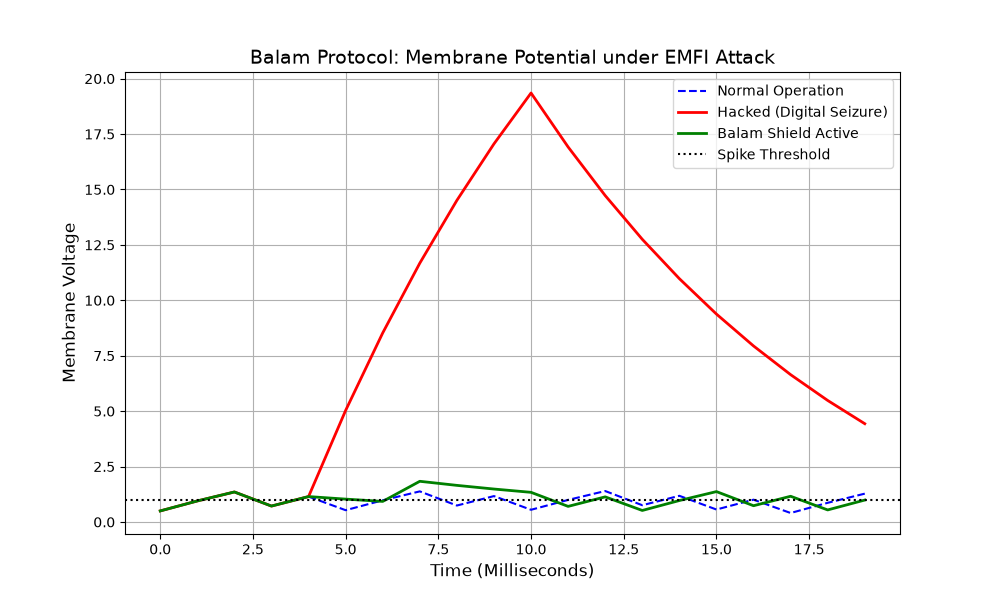
\includegraphics[width=0.8\textwidth]{balam_defense_plot.png}
    \caption{Membrane Potential under EMFI Attack vs. Balam Defense Active}
    \label{fig:defense_plot}
\end{figure}

\section{Experimental Results}
In a simulated environment utilizing PyTorch and snnTorch, a target SNN was subjected to a simulated 5.0v EMFI pulse. As demonstrated in Figure \ref{fig:defense_plot}, the unprotected neuron (red) exhibited catastrophic failure, spiking continuously. Upon activation of the Balam Protocol (green), the malicious pulse was mathematically neutralized, restoring the membrane potential to safe, operational levels.

\section{Conclusion and Future Work}
The software Proof of Concept confirms that runtime anomaly filtering is highly effective for SNNs. The next phase of Project Balam involves translating this PyTorch logic into VHDL/Verilog to test ultra-low latency execution directly on FPGA silicon.

\end{document}
